\documentclass{article}
\usepackage{styles/project_style} % Assuming you have this style file
\addbibresource{references/projects.bib}

% --- TITLE PAGE INFORMATION ---
\title{Introduction to Compartmental Models for COVID-19 Transmission}

\begin{document}
\maketitle

\section{What are Compartmental Models for COVID-19?}

Compartmental models are mathematical frameworks used to study the spread of infectious diseases like COVID-19. They divide a population into distinct groups, or ``compartments,'' based on disease status, such as Susceptible (S), Exposed (E), Infected (I), or Recovered (R). These models use differential equations or discrete-time rules to track how individuals move between compartments over time, driven by processes like infection, recovery, or interventions (e.g., vaccination). By simulating these dynamics, compartmental models help predict epidemic outcomes, evaluate intervention strategies, and understand key factors like transmission rates or incubation periods.

The SIR and SEIR models are foundational examples. The SIR model tracks Susceptible, Infected, and Recovered individuals, while the SEIR model adds an Exposed compartment to account for the incubation period, a critical feature for diseases like COVID-19. These models are widely used in epidemiology to study complex dynamics, such as how social distancing or vaccination can ``flatten the curve'' or prevent multiple epidemic waves.

\begin{figure}[htbp]
  \centering
  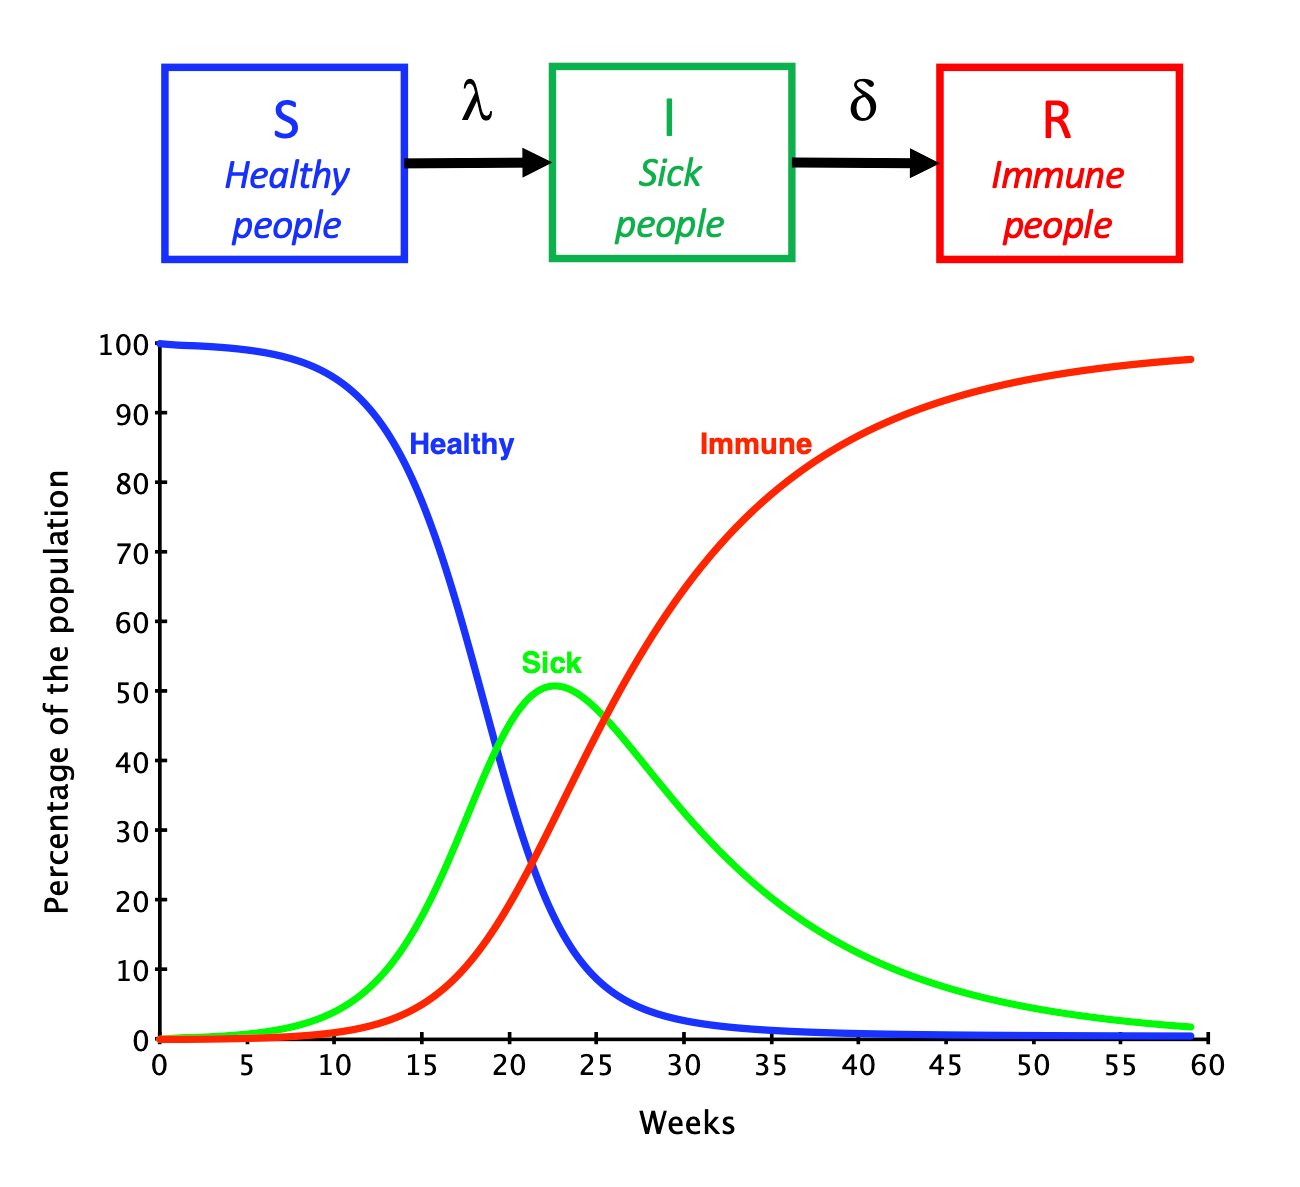
\includegraphics[width=0.4\textwidth]{lesson_3/images/sir_model.png}
  \caption{Schematic of the SIR model. The SIR model has three compartments: Susceptible (Healthy), Infectious (Sick) and Recovered (Immune). As the number of healthy people continually declines (blue dots), the number of sick people will first rise and then fall (green dots). The epidemic comes to an automatic halt. In the end, everybody has fallen ill and become immune (red dots).}
  \label{fig:seir-diagram}
\end{figure}

\subsection{Compartmental Models vs. Real-World Epidemiology}

Compartmental models, like SIR or SEIR, are simplified representations of disease spread. They focus on core processes (e.g., transmission, recovery) and assume a well-mixed population where everyone has an equal chance of interacting. In contrast, real-world epidemiology involves complex factors like spatial variation, heterogeneous contact patterns, specific viral strains, or detailed demographic data. Advanced models, such as agent-based simulations or network models, incorporate these details for more accurate predictions, similar to how wildfire management tools (e.g., FARSITE) go beyond the basic Forest Fire Model.

In this project, you will start with basic compartmental models (SIR and SEIR) and extend them to include COVID-19-specific features, such as asymptomatic transmission or intervention effects, to bridge the gap toward more realistic scenarios.

\subsection{How Do Compartmental Models Work?}

Compartmental models describe population dynamics using differential equations (continuous time) or difference equations (discrete time). Each compartment represents a fraction of the population, and transitions between compartments are governed by parameters like the transmission rate ($\beta$), recovery rate ($\gamma$), or incubation rate ($\sigma$). For example, in the SIR model, a Susceptible person becomes Infected at a rate proportional to the number of Infected individuals, while Infected individuals recover at a constant rate.

These models are solved numerically to simulate epidemic curves, showing how the number of Infected or Recovered individuals changes over time. By adjusting parameters or adding interventions (e.g., reducing $\beta$ to model social distancing), you can explore different scenarios, such as rapid outbreaks or controlled epidemics.

\section{Key Components and Rules}

The SIR and SEIR models operate on a population divided into compartments. Below are the key components and rules for each model.

\subsection{SIR Model}
The SIR model has three compartments:
\begin{itemize}
    \item \textbf{Susceptible (S):} Individuals who can contract the disease.
    \item \textbf{Infected (I):} Individuals who are infectious and can spread the disease.
    \item \textbf{Recovered (R):} Individuals who have recovered and are immune (or removed, e.g., deceased).
\end{itemize}

The dynamics are governed by:
\begin{itemize}
    \item \textbf{Infection:} A Susceptible individual becomes Infected at rate $\beta SI/N$, where $\beta$ is the transmission rate, $S$ and $I$ are the number of Susceptible and Infected individuals, and $N$ is the total population.
    \item \textbf{Recovery:} An Infected individual becomes Recovered at rate $\gamma I$, where $\gamma$ is the recovery rate.
\end{itemize}

The differential equations are:
\begin{align}
    \frac{dS}{dt} &= -\beta \frac{SI}{N}, \\
    \frac{dI}{dt} &= \beta \frac{SI}{N} - \gamma I, \\
    \frac{dR}{dt} &= \gamma I.
\end{align}

\subsection{SEIR Model}
The SEIR model adds an Exposed compartment:
\begin{itemize}
    \item \textbf{Exposed (E):} Individuals who are infected but not yet infectious (e.g., in the incubation period).
\end{itemize}

Additional rule:
\begin{itemize}
    \item \textbf{Progression:} An Exposed individual becomes Infected at rate $\sigma E$, where $\sigma$ is the rate of progression (inverse of the incubation period).
\end{itemize}

The differential equations are:
\begin{align}
    \frac{dS}{dt} &= -\beta \frac{SI}{N}, \\
    \frac{dE}{dt} &= \beta \frac{SI}{N} - \sigma E, \\
    \frac{dI}{dt} &= \sigma E - \gamma I, \\
    \frac{dR}{dt} &= \gamma I.
\end{align}

Parameters like $\beta$, $\gamma$, and $\sigma$ control the dynamics. For COVID-19, typical values might be $\beta \approx 0.3$ (daily transmission rate), $\gamma \approx 0.1$ (recovery in ~10 days), and $\sigma \approx 0.2$ (incubation period ~5 days).

\section{Why are Compartmental Models Important?}

Compartmental models are critical for understanding and managing infectious diseases like COVID-19. Their significance includes:
\begin{itemize}
    \item \textbf{Predicting Epidemic Trajectories:} Models forecast peak infection rates, healthcare demands, or epidemic duration, aiding resource planning.
    \item \textbf{Evaluating Interventions:} Simulations show how measures like vaccination, social distancing, or masking alter epidemic curves, guiding policy decisions.
    \item \textbf{Revealing Key Dynamics:} Models highlight critical factors, such as the role of asymptomatic transmission or the impact of early intervention.
    \item \textbf{Simplifying Complex Systems:} By focusing on core processes, models provide insights into complex dynamics, like multiple epidemic waves or endemic states.
    \item \textbf{Educational Value:} Implementing models teaches students about mathematical modeling, numerical methods, and epidemiology.
    \item \textbf{Inspiring Advanced Tools:} Simple models lay the groundwork for sophisticated tools, like agent-based models used in real-world pandemic response.
\end{itemize}

These models demonstrate how small changes, like reducing contact rates, can lead to significant outcomes, such as flattening the curve or preventing healthcare system overload.

\section{Algorithmic Representation}

The simulation of compartmental models typically involves solving the differential equations numerically (e.g., using Euler’s method or Runge-Kutta methods). The algorithm proceeds as follows:
\begin{enumerate}
    \item \textbf{Initialization:} Set initial conditions (e.g., $S \approx N$, $I = 1$, $E = 0$, $R = 0$), parameters ($\beta$, $\gamma$, $\sigma$), and time step $\Delta t$.
    \item \textbf{Time Evolution Loop:} For each time step:
        \begin{itemize}
            \item Compute transition rates (e.g., $\beta SI/N$ for infections).
            \item Update compartment sizes using the differential equations (e.g., $S(t + \Delta t) = S(t) - \beta \frac{SI}{N} \Delta t$).
            \item Store results for visualization (e.g., track $I(t)$ for the epidemic curve).
        \end{itemize}
    \item \textbf{Interventions (Optional):} Modify parameters at specific times (e.g., reduce $\beta$ to model social distancing). Note that this is only an optional step. Many model have fixed parameters. 
    \item \textbf{Visualization:} Plot compartment sizes over time to show epidemic curves.
\end{enumerate}

\section{ Implementation Example}
The following code demonstrates a basic implementation of the SI (Susceptible–Infected) model in MATLAB. This is the simplest type of compartmental model, where individuals can only transition from the Susceptible compartment to the Infected compartment. Recovery is not included, making it suitable for scenarios where infection persists indefinitely or for short-term spread estimation.

The model is implemented using Euler’s method, a straightforward numerical integration technique that approximates differential equations using finite time steps. This method is sufficient for simple models and educational purposes, although more accurate methods (e.g., Runge-Kutta) are recommended for larger or more sensitive systems.

The code is divided into three logical sections: initialization, simulation, and visualization. The first part initializes the parameters and sets up the simulation:

\begin{lstlisting}[caption={Initiation}]
% Parameters
beta = 0.3;       % infection rate
N = 1000;         % total population
I0 = 1;           % initial number of infected individuals
S0 = N - I0;      % initial number of susceptible individuals
t_max = 60;       % duration of simulation (days)
dt = 0.1;         % time step

% Time vector
t = 0:dt:t_max;
num_steps = length(t);

% Initialize S and I arrays
S = zeros(1, num_steps); I = zeros(1, num_steps);

% Set initial values
S(1) = S0; I(1) = I0;
\end{lstlisting}

Here, we define the transmission rate \texttt{beta}, the total population \texttt{N}, and the initial number of infected individuals. The rest of the population is considered susceptible. We also define the simulation time span and the numerical time step \texttt{dt}. The time vector and arrays to store compartment sizes are preallocated for efficiency. The second section performs the actual simulation:
\begin{lstlisting}[caption={Simulation loop}]
% Simulation loop 
for i = 2:num_steps
    dS = -beta * S(i-1) * I(i-1) / N;
    dI = -dS;  % because S + I = N
    S(i) = S(i-1) + dS * dt;
    I(i) = I(i-1) + dI * dt;
end
\end{lstlisting}
At each time step, we compute the change in susceptible and infected individuals using the SI model differential equations. Since there's no recovery, every infected individual remains infectious indefinitely. The decrease in susceptible individuals directly corresponds to the increase in infected individuals, preserving the total population size. Finally, the results are plotted:

\begin{lstlisting}[caption={Plotting}]
% Plot results
plot(t, S, 'b', 'LineWidth', 2);
hold on;
plot(t, I, 'r', 'LineWidth', 2);
xlabel('Time (days)'); ylabel('Number of individuals');
legend('Susceptible', 'Infected');
title('SI Model Simulation');
\end{lstlisting}
This produces a time series showing how the number of susceptible individuals decreases and the number of infected individuals increases over time. The steepness of the curve depends on the transmission rate \texttt{beta}. In real-world modeling, such output helps visualize epidemic progression and identify when an infection might reach its peak.

To model more realistic dynamics, such as recovery or an incubation period, additional compartments (e.g., Exposed or Recovered) and corresponding equations can be added. This can be efficiently handled in MATLAB using built-in solvers like \texttt{ode45}, which is particularly useful for larger models with more compartments and parameter changes over time.

\section{Literature}
\subsection{General introduction}
The topic is well discussed in several online resources. Wikipedia is a good starting point. There are several peer reviewed articles with introductory information. In addition several videos on YouTube on the topic. See:
\begin{itemize}
    \item \textcite{SIR_wiki}
     \item \textcite{SIR_AbouIsmail2020}
    \item \textcite{SIR_Tolles2020}
\end{itemize}

\subsection{Journal Club}
Compartment models were extensively used in modeling of Covid-19. Here are several papers that can be discussed in the Journal Club presentation.
\begin{itemize}
    \item \textcite{SIR_Bjrnstad2020}
   \item \textcite{SIR_Angulo2021}
    \item \textcite{SIR_Cooper2020}
    \item \textcite{SIR_He2020}

\end{itemize}


\section{Conclusion}
Compartmental models provide a framework for understanding the spread of infectious diseases like COVID-19. Through mathematical abstraction and numerical simulation, models such as SIR and SEIR enable to analyze key transmission dynamics, assess intervention strategies, and forecast epidemic trajectories. While these models simplify reality, they serve as a good starting point for more complex epidemiological tools. Their value lies not only in predictive insights but also in their educational clarity. 


\printbibliography

\end{document}
